\documentclass{standalone}
\usepackage{mintikz}

\begin{document}
\thispagestyle{empty}
\begin{tikzpicture}[]
    %\draw[thin, black!20] (0,0) grid (20,-20);
    \tikzset{header/.style={draw, rounded corners, fill=#1!20},
        header/.default={gray}}
    % Start left
    \begin{scope}
        %%%%%%%%%%%%%%%%%%%%%%%%%%%%%%%%%%%%%%%%%%%%%%%%%%%%%%%%%%%%%%%%%%%%%%%
        % Start SIMLIM
        \node[header=blue]
            (SIMLIB) at (0,0) {SIMLIB};
        \matrix[matrix of nodes,
            anchor=north,
            row sep=-1pt,
            column sep=-\pgflinewidth]
        (Msimlib) at ([shift={(0,-0.1)}]SIMLIB.south)
        {$z$ | & Date | & RADEC \\
        \vdots & \vdots & \vdots \\};
        %%%%%%%%%%%%%%%%%%%%%%%%%%%%%%%%%%%%%%%%%%%%%%%%%%%%%%%%%%%%%%%%%%%%%%%
        % START HOSTLIB
        \node[header=blue, below=12pt]
            (HOSTLIB) at (Msimlib.south) {HOSTLIB};
        \matrix[matrix of nodes, anchor=north,
            row sep=-1pt, column sep=-\pgflinewidth,
            text width=40pt, align=center,
            left delimiter=|,
            nodes={anchor=center, align=center}]
        (Mhostlib) at ([shift={(0,-0.1)}]HOSTLIB.south)
        {ID & $z$ & hostmass & $x_1$ & $c$ & $\Delta mag$ \\
        \vdots & \vdots & \vdots & \vdots & \vdots & \vdots\\
        \vdots & \vdots & \vdots & \vdots & \vdots & \vdots\\};
        % Vlines
        \foreach \n in {1, 3, 4, 5}{
            \draw[]
                (Mhostlib-1-\n.north east-|Mhostlib-3-\n.south east) |-
                (Mhostlib-3-\n.south east);}
        \draw[]
            (Mhostlib-2-2.north east-|Mhostlib-3-2.south east) |-
            (Mhostlib-3-2.south east);
        %%%%%%%%%%%%%%%%%%%%%%%%%%%%%%%%%%%%%%%%%%%%%%%%%%%%%%%%%%%%%%%%%%%%%%%
        % SIMLIB to HOSTLIB
        \draw[->]
            (Msimlib-2-1) to[bend right]
            (Mhostlib-1-2);
        % HOSTLIB z to hostmass
        \draw[->]
            ([shift={(3pt,0)}]Mhostlib-1-2.center) --
            ([shift={(-21pt,0)}]Mhostlib-1-3.center);
        %%%%%%%%%%%%%%%%%%%%%%%%%%%%%%%%%%%%%%%%%%%%%%%%%%%%%%%%%%%%%%%%%%%%%%%
        % WGTMAP
        \pgfplotstableread{../Data/PS1.txt} \wgttable
        \node[header=blue, below=12pt]
            (WEIGTHMAP) at (Mhostlib.south) {WEIGTHMAP};
            \begin{axis}[
                shift={($(WEIGTHMAP.south)+(0,-12pt)$)},
                anchor=north,
                xmin=8, xmax=12.3,
                ymin=0, ymax=1,
                xlabel=$M_{\rm host}$, ylabel=$P(M)$,
                axis lines=left,
                clip=false]
                \addplot[black, samples=500]
                    table[x=M, y=WGT] from \wgttable;
        \end{axis}
    % \coordinate (XS1) at (SIMLIB.east-|Mhostlib-1-6.east);
    % \len{(XS1)}{(SIMLIB.center)}{\xsa}
    % \node[] at (3,0) {\Huge \xsa};
    \end{scope}
    \begin{scope}[xshift=10cm]
        %%%%%%%%%%%%%%%%%%%%%%%%%%%%%%%%%%%%%%%%%%%%%%%%%%%%%%%%%%%%%%%%%%%%%%%
        % Start TRUE
        \node[header=green] (TRUE) at (0,0) {TRUE};
        %%%%%%%%%%%%%%%%%%%%%%%%%%%%%%%%%%%%%%%%%%%%%%%%%%%%%%%%%%%%%%%%%%%%%%%
        % M DIST from BP_lowz HOSTLIB
        \pgfplotstableread{../Data/mdist.txt} \mtable
        \begin{axis}[name=mdist, scale=0.5,
            yshift=-1cm, anchor=north, 
            xmin=6, xmax=14,
            ymin=0, ymax=0.6,
            xlabel=$M$, ylabel=$P$,
            axis lines=left,
            clip=false]
            \addplot[smooth, black]
                table[x=M, y=P] from \mtable;
        \end{axis}
        %%%%%%%%%%%%%%%%%%%%%%%%%%%%%%%%%%%%%%%%%%%%%%%%%%%%%%%%%%%%%%%%%%%%%%%
        % X1 DIST from basemodel
        \pgfplotstableread{../Data/basemodel.txt} \basetable
        \begin{axis}[name=x1dist, scale=0.5,
            at={(mdist.below south west)}, yshift=-0.3cm, anchor=north west, 
            xmin=-3, xmax=3,
            ymin=0, ymax=0.5,
            xlabel=$\bar{x_1}$, ylabel=$P$,
            axis lines=left,
            clip=false]
            \addplot[smooth, black]
                table[x=xlin, y=values] from \basetable;
        \end{axis}
        %%%%%%%%%%%%%%%%%%%%%%%%%%%%%%%%%%%%%%%%%%%%%%%%%%%%%%%%%%%%%%%%%%%%%%%
        % c DIST from stretchevol's asym with Scolnic 18 params:
        % -0.068, 0.034, 0.123
        \pgfplotstableread{../Data/casym.txt} \ctable
        \begin{axis}[name=cdist, scale=0.5,
            at={(x1dist.below south west)}, yshift=-0.3cm, anchor=north west,
            xmin=-0.3, xmax=0.3,
            ymin=0, ymax=5,
            xlabel=$\bar{c}$, ylabel=$P$,
            axis lines=left,
            clip=false]
            \addplot[smooth, black]
                table[x=clin, y=values] from \ctable;
        \end{axis}
        %%%%%%%%%%%%%%%%%%%%%%%%%%%%%%%%%%%%%%%%%%%%%%%%%%%%%%%%%%%%%%%%%%%%%%%
        % z DIST Rate from equation 6 of DES 2019 
        % https://arxiv.org/pdf/1811.02379.pdf
        \begin{axis}[name=zdist, scale=0.5,
            at={(cdist.below south west)}, yshift=-0.3cm, anchor=north west,
            xmin=0, xmax=1.2,
            ymin=0, ymax=7.5,
            xlabel=$\bar{z}$, ylabel=\# (1$^{-15}$),
            axis lines=left,
            clip=true]
            \addplot[smooth, black]
                {1.75*(1+x)^2.11};
        \end{axis}
        \node[right] (TS) at ([shift={(3,0)}]cdist.east)
        {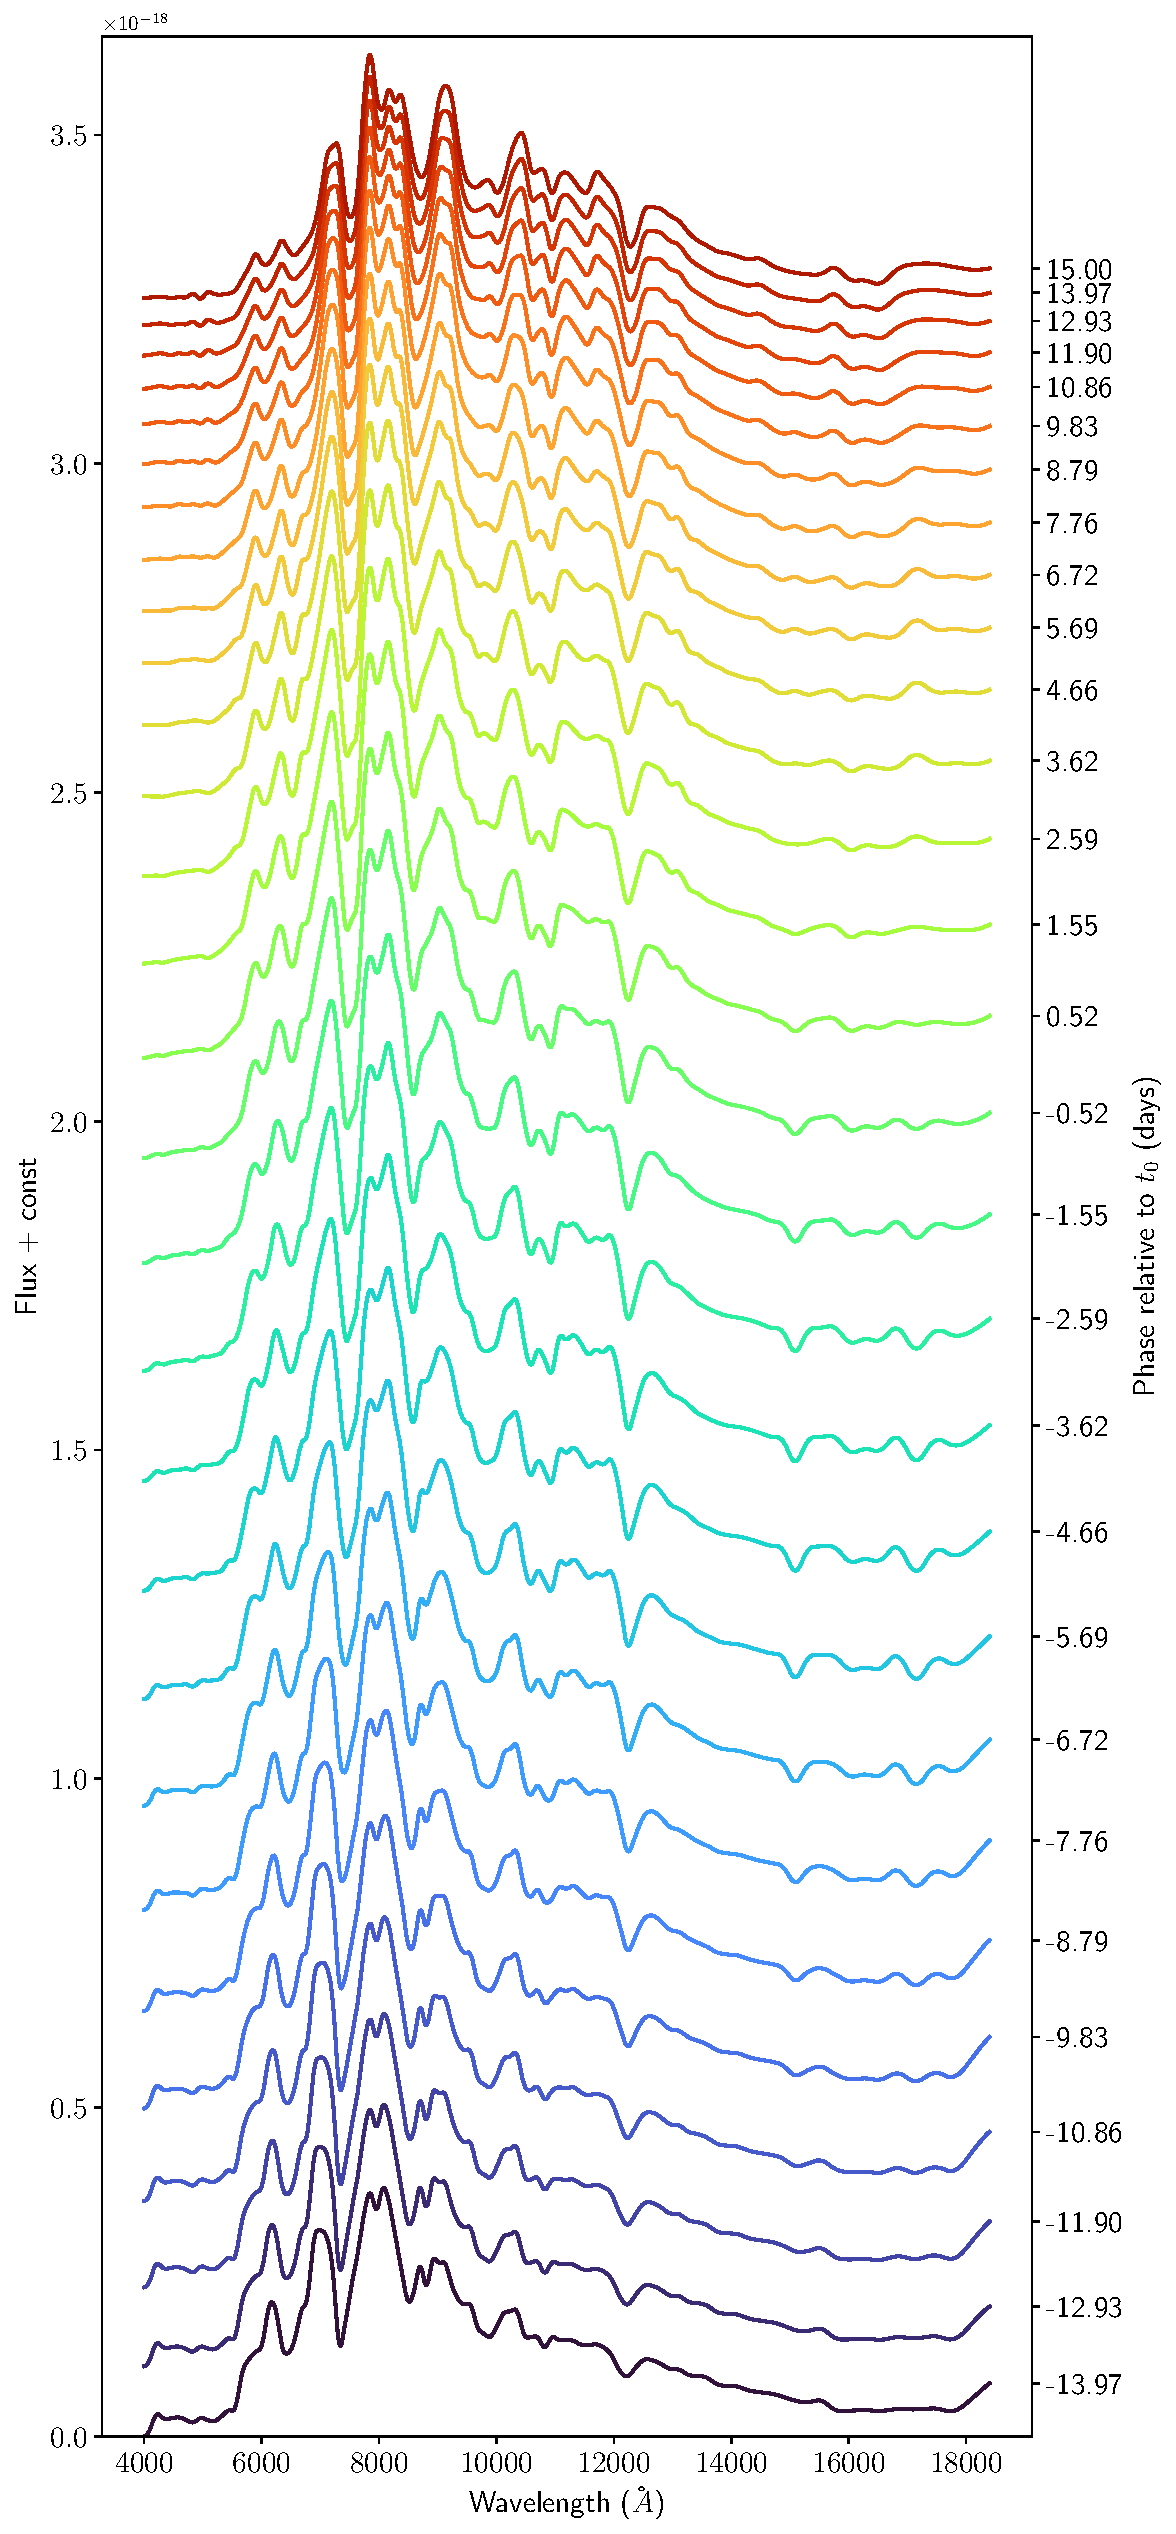
\includegraphics[scale=0.3]{timeseries.pdf}};
        \foreach \d/\y in {x1dist/0.2, cdist/0, zdist/-0.2}{
            \draw[->, >=stealth]
                (\d.east) --
                ([shift={(0,\y)}]TS.west);}
        \coordinate (Tleft) at (TS.east|-TRUE.north east);
        % \node[draw] at (Tleft) {Tleft};
    \end{scope}
    \begin{scope}[xshift=30cm]
        \node[header] (SURVEY) at (0,0) {SURVEY};
    \end{scope}
    % \begin{scope}[shift={(12,0)}]
    %     \node[header=blue] (SELECTION) at (0,0) {Selection};
    % \end{scope}
    % \begin{scope}[shift={(16,0)}]
    %     \node[header=red] (SIMRES) at (0,0) {Simulation propreties};
    % \end{scope}
    % \begin{scope}[shift={(20,0)}]
    %     \node[header=blue] (LCFIT) at (0,0) {LC fit};
    % \end{scope}
 \end{tikzpicture}
\end{document}
